
\chapter{内存与速度考量}

{
\tikzset{external/figure name/.add={}{memspeed_}}

\section{\TeX{} 的内存上限}
\label{sec:pgfplots:optimization}

只要正确配置 \TeX{} 的内存上限，\PGFPlots{} 就能排版包含数千个数据点的图。其运行时间大致与输入点数成正比。\footnote{事实上，运行时间是伪线性的：当点数大约达到 $100{,}000$ 时，会退化为二次增长。这一限制同样适用于 \PGF{} 路径的路径长度。此外，对堆叠图（stacked plots）而言，线性运行时间目前尚不可实现。}
%
\pgfplotsexpensiveexample
\begin{codeexample}[]
\begin{tikzpicture}
\begin{axis}[
    enlargelimits=0.01,
    title style={yshift=5pt},
    title=Scatter plot with $2250$ points,
]
    \addplot [
        blue,
        mark=*,
        only marks,
        mark options={scale=0.3},
    ] file [skip first]
        {plotdata/pgfplots_scatterdata3.dat};
\end{axis}
\end{tikzpicture}
\end{codeexample}

\pgfplotsexpensiveexample
\begin{codeexample}[]
\begin{tikzpicture}
\begin{axis}[
    enlarge x limits=0.03,
    title=Ornstein--Uhlenbeck sample
        ($13000$ time steps),
    xlabel=$t$,
]
    \addplot [blue] file {plotdata/ou.dat};
\end{axis}
\end{tikzpicture}
\end{codeexample}

\pgfplotsexpensiveexample
\begin{codeexample}[]
% huger graphs are possible; consider lualatex
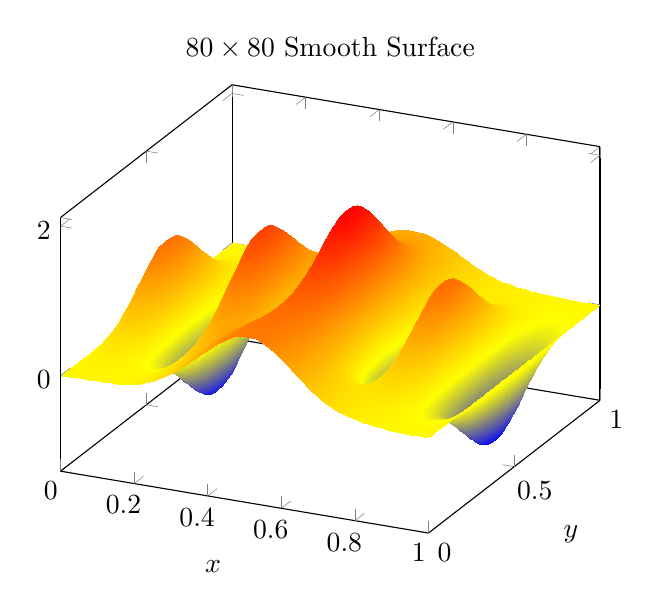
\begin{tikzpicture}
\begin{axis}[
    title=$80 \times 80$ Smooth Surface,
    xlabel=$x$,
    ylabel=$y$,
]
  \addplot3 [surf,samples=80,shader=interp,domain=0:1]
        {sin(deg(8*pi*x))* exp(-20*(y-0.5)^2)
        + exp(-(x-0.5)^2*30
            - (y-0.25)^2 - (x-0.5)*(y-0.25))};
\end{axis}
\end{tikzpicture}
\end{codeexample}

\PGFPlots{} 完全依赖 \TeX{} 完成所有排版工作。它使用 \PGF{} 的前端层（front-end layer）和基础层（basic layer）来执行所有绘图操作。对于复杂的图，这可能需要花费一些时间，你可以参阅第~\ref{cha:pgfplots:importexport} 章，了解如何将单个图导出到外部图形文件。外部化（externalization）是减少排版时间的最佳方式。

然而，对于包含大量数据点的大规模图，很容易触及 \TeX{} 自身能力的上限。


\section{内存限制}

大多数 \TeX{} 发行版的默认设置都相当保守，因此可能需要调整它们。

通常，日志文件或最终的错误消息会包含一段关于已使用资源的摘要，从而提示需要增大哪一个参数。


\subsection{Lua\LaTeX{}}

一个效果相当不错的解决方案是切换 \LaTeX{} 可执行程序：如果你使用的是一个较完善的 \TeX{} 发行版，那么它应该已经附带了 |lualatex| 可执行程序。它采用动态内存分配，因此通常对任何 \PGFPlots{} 坐标轴都有足够的内存可用。

Lua\LaTeX{} 可执行程序 |lualatex| 与 |pdflatex| 几乎完全兼容。

这种方法适用于任何平台。


\subsection{MiK\TeX{}}

如果你正在使用 MiK\TeX{}，并且不想（或不能）切换到 |lualatex|，可以按如下步骤操作。

对于 MiK\TeX{}，可以通过两种方式增大内存上限。第一种是使用命令行开关：
%
\begin{codeexample}[code only]
pdflatex
    --stack-size=n --save-size=n
    --main-memory=n --extra-mem-top=n --extra-mem-bot=n
    --pool-size=n --max-strings=n
\end{codeexample}
%
\noindent 如果 MiK\TeX{} 出现内存不足，请调整这些设置。通常，我们不会手动调用 |pdflatex|：有一个开发辅助工具会负责所有调用，因此需要调整的是它。

有时，永久修改 MiK\TeX{} 配置文件可能更好，例如可以避免每次重新配置 \TeX{} 开发程序。这可以通过下面的命令实现
%
\begin{codeexample}[code only]
initexmf --edit-config-file=pdflatex
\end{codeexample}
%
\noindent 该命令既可以在 Windows 的命令提示符中输入，也可以通过「开始 $\gg$ 运行」执行。执行后，系统会用编辑器打开相应的配置文件。一个示例配置文件可以是
%
\begin{codeexample}[code only]
main_memory=90000000
save_size=80000
\end{codeexample}
%
或者也可以输入下面列出的任意一项配置。感谢 ``LeSpocky'' 提供的文档：

\url{http://blog.antiblau.de/2009/04/21/speicherlimits-von-miktex-erhoehen}.


\subsection{\TeX{}Live 或类似发行版}

除了切换到 |lualatex| 之外，你还可以按如下方式操作，以保留现有的 |dvips| 或 |pdflatex| 工作流。

对于 Unix 安装，需要调整配置文件。可以按如下步骤进行：
%
\begin{enumerate}
    \item 在你的系统上找到 |texmf.cnf|。在我的 Ubuntu 安装中，它位于

        |/usr/share/texmf/web2c/texmf.cnf|。
    \item 可以直接修改 |texmf.cnf|，也可以把它复制到某个方便的位置。如果你选择复制，步骤如下：
        %
        \begin{itemize}
            \item 在你本地的副本中只保留被修改的条目，以减少冲突。\TeX{} 总是会读取其搜索路径中找到的 \emph{所有} 配置文件。
            \item 调整搜索路径，使其能找到你的本地副本。这可以通过环境变量 |TEXMFCNF| 来完成。假设你的本地副本位于 |~/texmf/mytexcnf/texmf.cnf|，则可以写
                %
\begin{codeexample}[code only]
export TEXMFCNF=~/texmf/mytexcnf:
\end{codeexample}
                %
                这样就会先在你的目录中搜索，然后再搜索所有其他系统目录。
        \end{itemize}
    \item 你应当修改以下条目
        %
\begin{codeexample}[code only]
main_memory = n
extra_mem_top = n
extra_mem_bot = n
max_strings = n
param_size = n
save_size = n
stack_size = n
\end{codeexample}
        %
        日志文件通常会包含关于需要增大哪一个参数的信息。
\end{enumerate}
%
下面给出一个此类配置文件的示例。它会修改内存上限。
%
\begin{enumerate}
    \item 创建文件 |~/texmf/mytexcnf/texmf.cnf|（如必要，也一并创建相应的路径）。
        %
\begin{codeexample}[code only]
% newly created file ~/texmf/mytexcnf/texmf.cnf:
% If you want to change some of these sizes only for a certain TeX
% variant, the usual dot notation works, e.g.,
% main_memory.hugetex = 20000000
main_memory = 230000000 % words of inimemory available; also applies to inimf&mp
extra_mem_top = 10000000     % extra high memory for chars, tokens, etc.
extra_mem_bot = 10000000     % extra low memory for boxes, glue, breakpoints, etc.
save_size = 150000    % for saving values outside current group
stack_size = 150000    % simultaneous input sources

% Max number of characters in all strings, including all error messages,
% help texts, font names, control sequences.  These values apply to TeX and MP.
%pool_size = 1250000
% Minimum pool space after TeX/MP's own strings; must be at least
% 25000 less than pool_size, but doesn't need to be nearly that large.
%string_vacancies = 90000
% Maximum number of strings.
%max_strings = 100000
% min pool space left after loading .fmt
%pool_free = 47500
\end{codeexample}
        %
    \item 运行 |texhash|，让 \TeX{} 更新它的 |~/texmf/ls-R| 数据库。
    \item 创建环境变量 |TEXMFCNF|，并将其值设为 `|~/texmf/mytexcnf:|'（注意末尾的 `|:|'！）。在我的 Linux 系统上，可以通过向 |~/.bashrc| 添加
        %
\begin{codeexample}[code only]
export TEXMFCNF=~/texmf/mytexcnf:
\end{codeexample}
        %
        来实现。
\end{enumerate}

遗憾的是，\TeX{} 不允许任意设置内存上限：可执行程序中硬编码了一个上界。


\section{减少排版时间}

\PGFPlots{} 会进行大量计算，从抽象的坐标计算一直到由 \PGF{} 实现的底层 |.pdf| 绘图命令。对于复杂的图，这可能需要相当长的时间——尤其是 3D 图。


\subsection{LUA}

如果你使用 |compat=1.12|（或更新版本），并通过 |lualatex| 编译文档，\PGFPlots{} 就会启用其 |lua backend|。这一开关能减少生成输出文件所需的时间，对 3D 图尤其明显。

\begin{pgfplotskey}{lua backend=\mchoice{true,false} (initially true)}
    如果 |lua backend| 处于活动状态，并且文档是通过 |lualatex| 处理的，\PGFPlots{} 就会启用可扩展性与性能改进；它产生的输出与不启用时相同，但耗时更少，并且具有更智能的内存管理。

    该特性依赖于用快速脚本语言 \lua 对 \PGFPlots{} 的部分重新实现。要从中受益，你需要
    %
    \begin{enumerate}
        \item 在导言区写入 |compat=1.12|（或更新版本），并且
        \item 使用 |lualatex| 来编译你的 |.tex| 文件（或者至少编译那些包含 \PGFPlots{} 图的文件）。
    \end{enumerate}

    使用该特性后，生成曲面图所需的时间可以缩减到纯 \TeX{} 实现（即 |pdflatex|）所需时间的 25\%--50\%。其他类型的图同样会从中受益。

    |lua backend| 以两种方式工作：第一，用更快的 \lua 对应实现替换若干独立的子程序。这相对通用。第二，用等价的 \lua 实现替换整个处理步骤。%
    %
    \footnote{
        第一种方式的一个例子是：每当 \PGFPlots{} 在其 |colormap| 中进行查找时，它就把控制权转交给 |lua backend|，并将结果立即传回给 \TeX{}。主控制流仍然位于较慢的 \TeX{} 实现中。第二种方式的一个例子是 \texttt{\textbackslash addplot expression}：\PGFPlots{} 会把数学表达式以及所有相关的输入参数（包括 \texttt{samples} 和 \texttt{domain}）拷贝到 \texttt{lua backend}。然后，\texttt{lua backend} 会执行所有循环并收集坐标，最终把这些坐标交给 \pgfname{} 的（\TeX{}）实现。这样，控制流就位于快速的 \lua{} 解释器中。
    }
    \PGFPlots{} 1.12 为重要且耗时的操作提供了 \lua{} 实现。只要可能，就会使用这一实现。然而，它目前只覆盖了部分功能：\PGFPlots{} 的某些特性尚不被 \lua{} 后端支持。在这种情况下，它会自动关闭，并回退使用 \TeX{} 实现。

    |lua backend| 还会继续扩展，以获得更多性能提升并覆盖更多特性。如果你想查看 |lua backend| 是否在你的图中被（去）激活，请参考 |lua debug|。

    请注意，|lua backend| 使用了一个不同的、精度更高的数学引擎。因此，与 |pdflatex| 生成的输出相比，图的外观可能会出现一些无关紧要的像素差异。一般建议固定使用其中一种方式来生成文档，即要么使用 |lualatex|，\emph{要么}使用 |pdflatex|。由于 |lua backend| 的存在，从一种方式迁移到另一种方式可能会改变你文档的外观。

    最终，\PGFPlots{} 可能会加入一些计算开销较大的特性，这些特性只能作为 |lua backend| 的一部分实现，没有它将不可用。

    请注意，|lua backend| 需要一个至少支持 \lua~5.2 的 \TeX{} 发行版（例如 \TeX{}Live 2014）。如果你的 |lualatex| 附带的是更老版本的 \lua{} 解释器，它会自动停用。

    下面是一些如何从 |lua backend| 受益的指南：
    %
    \begin{itemize}
        \item 涉及宏定义的数学表达式在 |lua backend| 中不可用。最佳实践：优先使用 |declare function| 而不是宏常量：
            %
\begin{codeexample}[]
\begin{tikzpicture}
\begin{axis}[
    small,
    title=Do,
    samples=2,
]
    \addplot+ [
        declare function={C=4;}
    ] {C*x};
\end{axis}
\end{tikzpicture}
\end{codeexample}

\begin{codeexample}[]
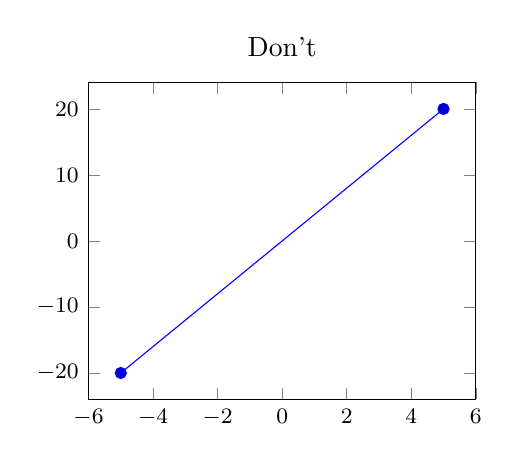
\begin{tikzpicture}
\begin{axis}[
    small,
    title=Don't,
    samples=2,
]
        \def\constantC{4}
    \addplot {\constantC*x};
\end{axis}
\end{tikzpicture}
\end{codeexample}

            两者在语义上是等价的，但由于 \lua{} 无法解释 \TeX{} 宏，它会拒绝处理「Don't」这一情形。「Don't」情形会产生一条日志消息
            %
\begin{verbatim}
Package pgfplots info on input line 16: Deactivating LUA version of
plot expression for plot 0 (type 'pgfplothandlerlineto'):
y expression '\constantC *x' contains a TeX macro.
\end{verbatim}
            %
        \item 任何需要「原生」\TeX{} 代码的操作在 |lua backend| 中都不可用。这包括 |x filter/.code={...}|，因为 |/.code| 无法映射到 \lua。最佳实践：优先使用 |x filter/.expression| 而不是 |x filter/.code|：
            %
\begin{codeexample}[]
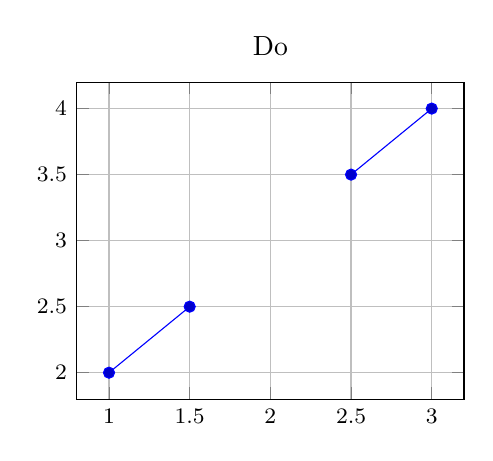
\begin{tikzpicture}
    \begin{axis}[small,grid=major,title=Do]
    \addplot+ [
        unbounded coords=jump,
        y filter/.expression={y==3 ? nan : y},
    ] table {
        x   y
        1   2
        1.5 2.5
        2   3
        2.5 3.5
        3   4
    };
    \end{axis}
\end{tikzpicture}
\end{codeexample}
            %
        \item 绘图表达式可以完全在 \lua 中处理；其他所有输入坐标类型仍由 \TeX{} 读取数值后再交给 \lua。
        \item 还有若干操作计划在未来版本中加入 |lua backend| 支持。
    \end{itemize}
\end{pgfplotskey}

\begin{pgfplotskeylist}{%
    lua debug,
    lua debug=\mchoice{false,off,off and silent,verbose,compileerror}%
}
    通常，|lua backend| 是静默工作的：\PGFPlots{} 自行决定它是否处于活动状态、是否支持当前操作，并据此继续执行。如果两个条件都满足，就会把控制权转交给 |lua backend|。如果其中一个不满足，它会自动回退到旧的 \TeX{} 实现。因此，你无法立即感知到它的存在，只有编译图片所需的时间会有所不同。

    该键用于控制：当 |lua backend| 处于活动状态、但由于遇到了不支持的特性而无法使用时，\PGFPlots{} 应如何处理。

    选项 \declaretext{false} 和 \declaretext{off} 会关闭 \lua{} 调试。在这种情况下，\PGFPlots{} \emph{仅}在使用了 \TeX{} 实现而不是 |lua backend| 时才写入日志消息。此外，它只会把消息写入 |.log| 文件（而不会写入控制台输出）。

    选项 \declaretext{off and silent} 既不写信息消息，也不写调试消息：它与 |off| 相同，只是在使用了 \TeX{} 实现时不再写日志消息。这是信息量最少的选项。

    选项 \declaretext{verbose} 还会把成功消息写入 |.log| 文件（不写入控制台）。

    选项 \declaretext{compileerror} 会在 |lua backend| 处于活动状态、但不支持当前图或绘图时中止编译。

    请注意，\PGFPlots{} 可能附带一些开销较大的受限操作，这些操作只能在 |lua backend| 中使用。如果由于某种原因无法使用 |lua backend|，这些条目将导致编译错误。
\end{pgfplotskeylist}


\subsection{每个图只编译一次}

减少排版时间的一种方法是：让 \PGF{} 在一次运行中为一部分（或全部）图形生成独立的临时 |.pdf|（或 |.eps|）文档，并在后续运行中复用这些临时图片。对于 \PGFPlots{} 而言，这是减少较大文档排版时间最有效的方式。可以通过第~\ref{sec:pgfplots:export} 节中描述的 |external| 库来实现。

}
